
\newpage
\section{Introducción}
El presente informe final tiene como propósito documentar la experiencia de prácticas preprofesionales realizada en la Oficina de \InstitucionNombre. Estas prácticas permitieron aplicar los conocimientos adquiridos durante la formación en Ingeniería de Sistemas en un entorno profesional, participando en el análisis, diseño, desarrollo y documentación de funcionalidades para el sistema de gestión de proyectos de la institución.

Durante el periodo de prácticas, el trabajo se desarrolló mediante un flujo iterativo e incremental. Para cada funcionalidad se elaboraba una propuesta de diseño, se presentaba al encargado de la oficina, se implementaba y posteriormente se realizaban los ajustes necesarios de acuerdo con la retroalimentación recibida. De esta manera, el informe presenta las actividades realizadas, los resultados obtenidos y las evidencias correspondientes al periodo comprendido entre el 15 de abril y el 15 de agosto de 2025.

El documento se organiza de la siguiente manera: primero se presentan la introducción, el marco legal y los objetivos de las prácticas; luego se desarrolla la parte informativa y la descripción del centro de prácticas. Posteriormente, se presenta el cumplimiento progresivo del plan, las tareas realizadas y los resultados obtenidos. Finalmente, se incluyen las conclusiones, recomendaciones, referencias y anexos.

\section{Marco legal}
\subsection{Ley Universitaria Nro. 30220}
La Ley Universitaria N° 30220, promulgada el 9 de julio de 2014, establece en su Artículo 49 que las universidades deben promover las Prácticas Pre - Profesionales de sus estudiantes con el objetivo de vincular la formación académica con la actividad laboral y productiva del país. El Artículo 90 dispone que los programas de estudio incluyan periodos de prácticas que fortalezcan la formación integral del egresado y faciliten su inserción al mercado laboral mediante el desarrollo de competencias aplicadas.

\subsection{Estatuto de la Universidad Nacional del Altiplano}
El Estatuto de la Universidad Nacional del Altiplano Puno, en concordancia con la Ley Universitaria N° 30220, establece que la formación profesional de los estudiantes debe articular los conocimientos teóricos con la experiencia práctica. Dispone que las Escuelas Profesionales organicen y supervisen las prácticas Pre - Profesionales como requisito para la obtención del grado de bachiller, garantizando el acompañamiento docente y que las actividades correspondan al perfil de la carrera profesional.

\subsection{Reglamento de Prácticas Pre - Profesionales}
El Reglamento de Prácticas Pre - Profesionales de la Escuela Profesional de Ingeniería de Sistemas (Código RG-001-FIMEES-P29-R, versión V01, vigente desde el 05 de agosto de 2024) regula el proceso de inscripción, desarrollo, supervisión y evaluación de las prácticas. Establece una duración mínima de cuatro meses, define los roles del practicante, el jefe del área receptora y el docente supervisor, y fija los instrumentos oficiales de evaluación (actitudinal, desempeño y rúbrica de sustentación) que deben completarse para la aprobación del informe final.

\section{Objetivos de las prácticas preprofesionales}
\subsection{Objetivo general}
Aplicar los conocimientos adquiridos en la Escuela Profesional de Ingeniería de Sistemas mediante el análisis, diseño, desarrollo y documentación de funcionalidades para el sistema de gestión de proyectos de la Oficina de \InstitucionNombre.

\subsection{Objetivos específicos}
\begin{enumerate}
    \item Analizar los requerimientos del sistema de gestión de proyectos de acuerdo con las necesidades de las subunidades de la institución.
    \item Diseñar las funcionalidades y sus interfaces antes de su implementación.
    \item Presentar las propuestas de diseño al encargado de la oficina para recibir observaciones y retroalimentación.
    \item Implementar funcionalidades del sistema y realizar los ajustes correspondientes según la retroalimentación recibida.
    \item Documentar las actividades, los resultados y las evidencias del proceso de desarrollo.
\end{enumerate}

\section{Parte Informativa}
\subsection{Datos del practicante}
\begin{table}[htb!]
    \centering
    \renewcommand{\arraystretch}{1.3}

    \begin{tabularx}{\linewidth}{
        @{}
        >{\raggedright\arraybackslash}p{0.34\linewidth}
        @{\hspace{0.5em}:\hspace{0.5em}}
        >{\raggedright\arraybackslash}X
        @{}
    }
        Apellidos y nombres & \PracticanteNombre \\
        Código & \PracticanteCodigo \\
        Especialidad de prácticas & \PracticanteEspecialidad \\
        Modalidad de prácticas & Presencial \\
        Facultad & \PracticanteFacultad \\
        Promoción & \PracticantePromocion \\
    \end{tabularx}
\end{table}

% Centro de prácticas
\subsection{Centro de practicas}
\begin{table}[htb!]
    \centering
    \renewcommand{\arraystretch}{1.3}
    \begin{tabularx}{\linewidth}{
        @{}
        >{\raggedright\arraybackslash}p{0.34\linewidth}
        @{\hspace{0.5em}:\hspace{0.5em}}
        >{\raggedright\arraybackslash}X
        @{}
    }
        Nombre de la entidad & \InstitucionNombre \\
        Dependencia/Oficina & \InstitucionOficina \\
        Jefe inmediato & \InstitucionJefa \\
        Modalidad de prácticas & Presencial \\
    \end{tabularx}
\end{table}
\subsection{Periodo de prácticas}
\begin{table}[htb!]
    \centering
    \renewcommand{\arraystretch}{1.3}
    \begin{tabularx}{\linewidth}{
        @{}
        >{\raggedright\arraybackslash}p{0.34\linewidth}
        @{\hspace{0.5em}:\hspace{0.5em}}
        >{\raggedright\arraybackslash}X
        @{}
    }
        Fecha de inicio & \FechaInicio \\
        Fecha de Culminación & \FechaFin \\
        Duración & 4 meses \\
    \end{tabularx}
\end{table}
\subsection{Docente de prácticas}
\Precidente

\section{Descripción del centro de prácticas}
\subsection{Nombre de la institución}
Oficina: \InstitucionNombre

\subsection{Dirección del centro de prácticas}
\CentroDireccion

\subsection{Teléfono, fax, página web, correo electrónico}
\href{\SitioWeb}{\SitioWeb}

\begin{table}[htb!]
    \centering
    \renewcommand{\arraystretch}{1.3}
    \begin{tabularx}{\linewidth}{
        @{}
        >{\raggedright\arraybackslash}p{0.34\linewidth}
        @{\hspace{0.5em}:\hspace{0.5em}}
        >{\raggedright\arraybackslash}X
        @{}
    }
        \TelefonoMelissa & Ing Melissa (Encargada del proyecto). \\
        \TelefonoJefa & \InstitucionJefa (Directora de la oficina DPSEC). \\
        \TelefonoOficina & Oficina DPSEC (secretaria) \\
    \end{tabularx}
\end{table}

\subsection{Visión}	
La Dirección de Proyección Social y Extensión Cultural fortalece el desarrollo de la región, bajo los principios de la ciencia, la tecnología, los valores culturales y la investigación en el marco de una responsabilidad social sostenible.

\subsection{Misión}
La Dirección de Proyección Social y Extensión Cultural es generadora de la interacción con la comunidad para el desarrollo regional a través de la ciencia, la tecnología y las expresiones culturales como parte de la labor académica y de investigación en el marco de la proyección social y extensión cultural sostenible.

\subsection{Valores institucionales}
\begin{enumerate}
    \item \textbf{Responsabilidad:} Compromiso con el cumplimiento de las obligaciones y tareas asignadas.
    \item \textbf{Respeto:} Reconocimiento y consideración hacia las personas, sus ideas y derechos.
    \item \textbf{Integridad:} Actuar con honestidad y ética en todas las acciones.
    \item \textbf{Compromiso Social:} Participación activa en el desarrollo y bienestar de la comunidad.
    \item \textbf{Excelencia:} Búsqueda constante de la calidad en el desempeño académico y profesional.
    
\end{enumerate}

\subsection{Objetivos de la institución}
Promover, organizar, dirigir, supervisar y evaluar las actividades en el marco de la proyección social, extensión cultural y dimensión ambiental sostenible de la universidad, orientados hacia la comunidad, con el fin de coadyuvar al desarrollo e inserción laboral, re-valorando su identidad cultural.

\subsection{Actividad principal de la institución}
La Dirección de Proyección Social y Extensión Cultural, es un órgano dependiente del Vicerrectorado Académico, responsable de promover, organizar, dirigir y supervisar las actividades en el marco del desarrollo sostenible de Proyección Social y Extensión Cultural de la universidad, orientados hacia la comunidad, con el fin de coadyuvar al desarrollo de la región, revalorando la identidad cultural.


\subsection{Funciones de la oficina de prácticas}
\begin{enumerate}
    \item Proponer reglamentos o directivas de su competencia, para aprobación y aplicación.
    \item Revalorar, promover y preservar la riqueza cultural de la región.   
    \item Promover y apoyar a los estudiantes en sus actividades culturales.	
    \item Vincular la universidad con la sociedad a través de actividades de extensión cultural y proyección social.
    \item Programar, organizar y ejecutar eventos científicos, tecnológicos y culturales que contribuyan al desarrollo de la región.
    \item Coordinar, ejecutar y supervisar los programas y proyectos de proyección social y extensión cultural universitaria.
    \item Establecer la racionalidad de la calendarización de las actividades culturales y deportivas de manera que no afecten el desarrollo de las actividades académicas.
    \item Proponer la política, objetivos, acciones estratégicas de Proyección Social y Extensión Cultural de la Universidad, en coordinación con las unidades orgánicas de la universidad.
    \item Diseñar y ejecutar planes, programas, estrategias y acciones para consolidar la vinculación y el soporte necesario para los graduandos de la UNA-PUNO.
    \item Desarrollar programas de apoyo en coordinación con las facultades a través de la extensión cultural y proyección social que permitan proponer soluciones viables y sustentables a problemas de la región.
    \item Realizar investigaciones relacionadas con la situación profesional, académica y laboral de los exalumnos de la universidad y de la relación entre el empleo y la oferta académica en su zona de influencia.
    \item Planificar, dirigir, ejecutar, supervisar y evaluar las actividades de mantenimiento de infraestructura ambiental, manejo adecuado de residuos, sensibilización y educación ambiental en la Universidad.
    \item Contribuir en la formulación de la política académica de la Universidad en materia de promoción y fomento del desarrollo sostenible, gestión de riesgos y adaptación al cambio climático y protección y conservación del medio ambiente.
    \item Registrar y administrar información y estadísticas de los graduados de la universidad, a través de un sistema informático integral, que permita procesar y obtener del mismo, una serie de reportes a fines a esta área para la toma de decisiones y la elaboración de planes de mejora.
    \item Proponer la suscripción de convenios de proyección social y extensión cultural de facultades con instituciones públicas, privadas y organizaciones de base, con la finalidad de objetivar los diferentes planes de desarrollo de estas organizaciones.
    \item Fomentar y promover la educación ambiental, participación en programas de gestión ambiental, proyectos de desarrollo y conservación del medio ambiente en todos los niveles dentro y fuera de la Universidad.
    \item Formular y proponer la aplicación de normas ambientales que promuevan la conservación del medio ambiente y adaptación al cambio climático en las actividades bajo la competencia de la Universidad.
    \item Las demás que le asigne el Vicerrectorado Académico o la Alta Dirección en el ámbito de su competencia.
    
\end{enumerate}

\subsection{Funciones específicas del practicante}


\subsection{Organigrama de la institución}
\begin{figure}[h] % Entorno para manejar imágenes
    \centering % Centra la imagen
    \caption{Organigrama de la institución} % Pie de la imagen
    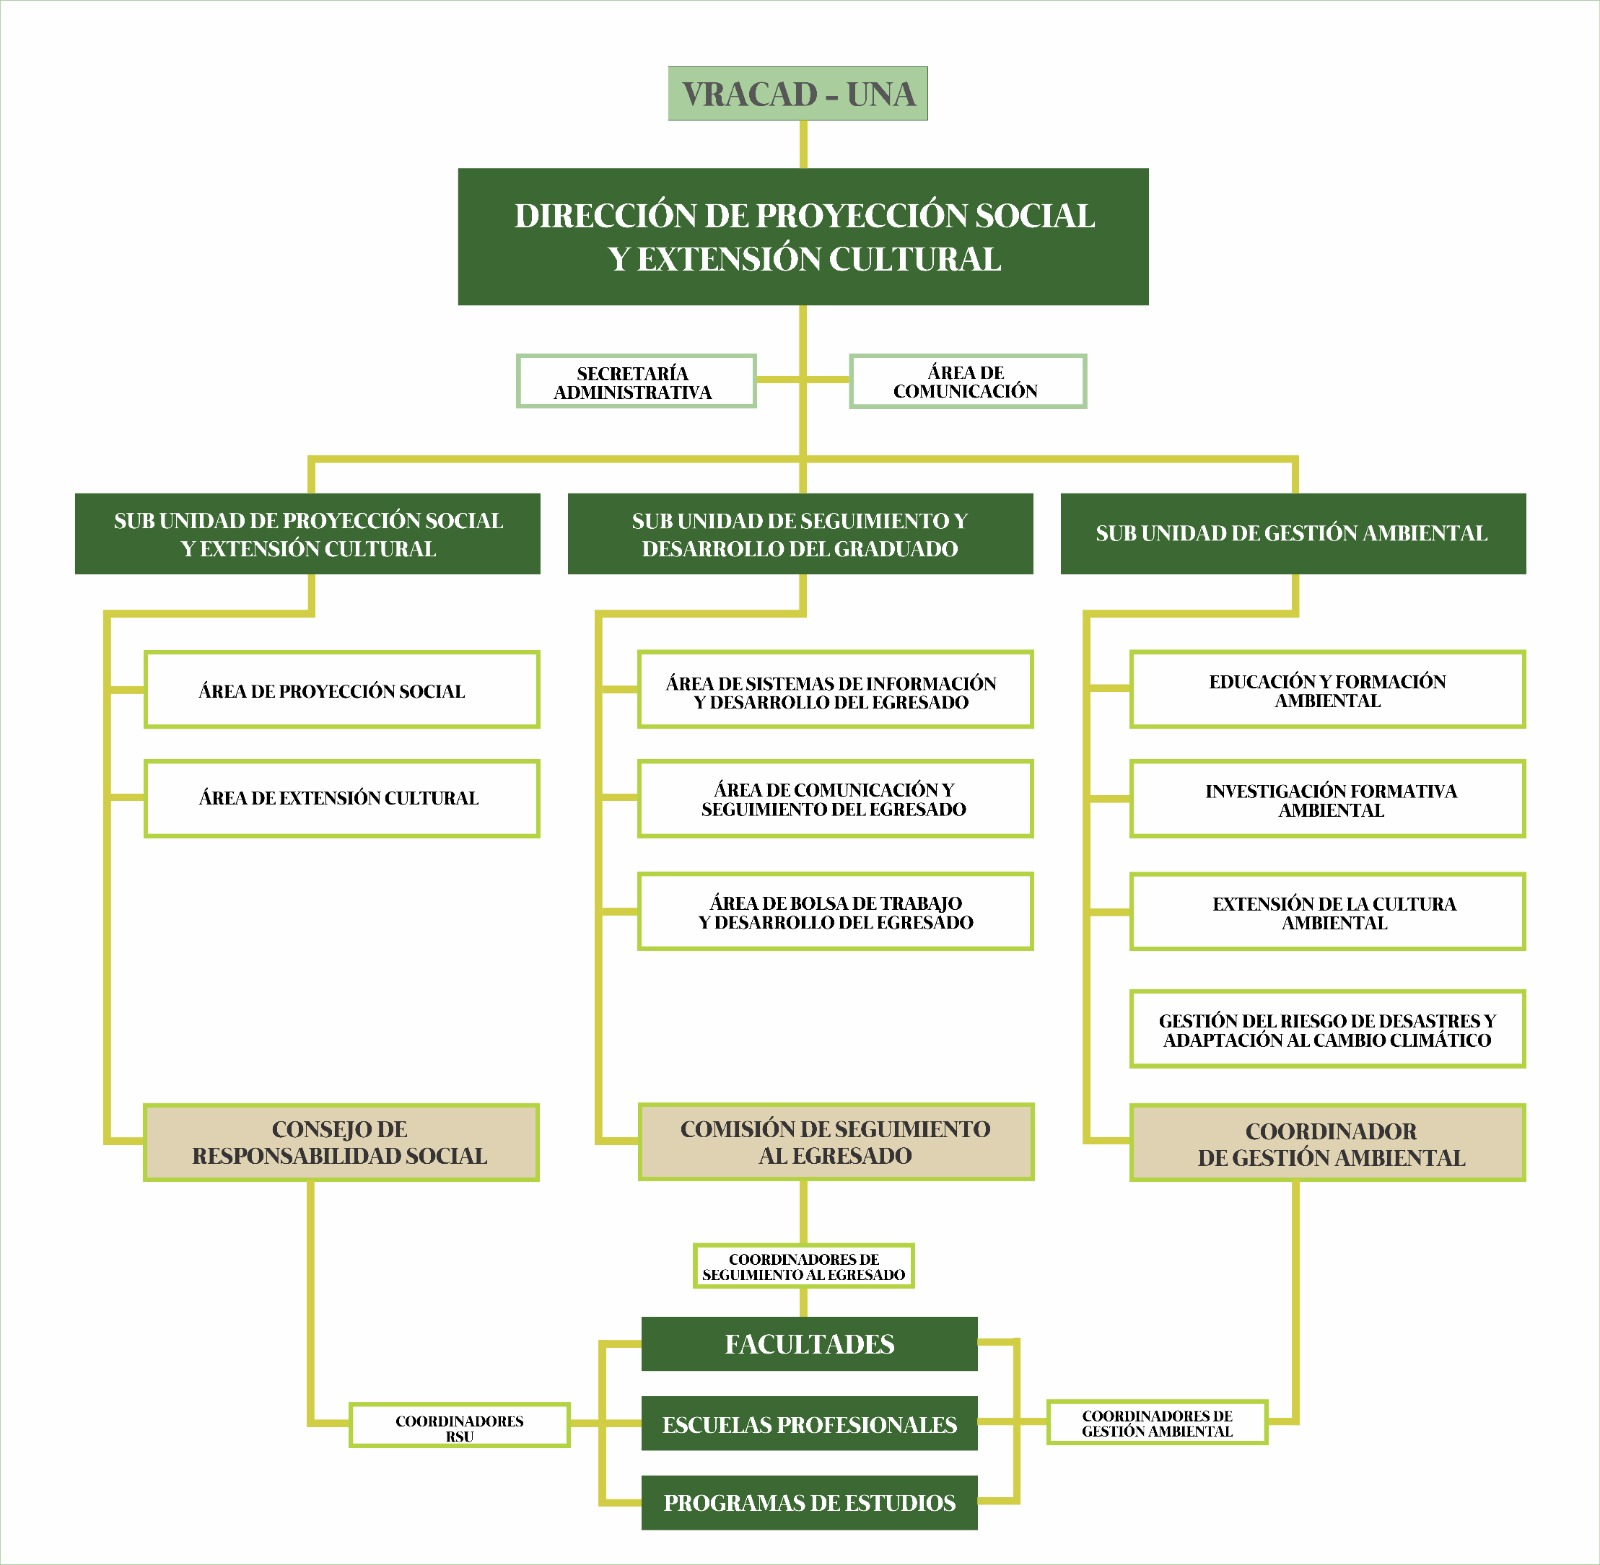
\includegraphics[width=0.8\textwidth]{assets/imagenes/estructura.jpeg} % Incluye la imagen y ajusta su ancho
    \label{fig:organigrama} % Etiqueta para referenciar
\end{figure}
\FloatBarrier
